\documentclass[10pt,letterpaper]{article}
\usepackage[english]{babel}
\usepackage{graphicx}
\usepackage[margin=2cm]{geometry}

\usepackage{subcaption}
\usepackage{mathtools}
\usepackage{amsfonts}
\usepackage{amsmath}
\usepackage{amssymb}
\usepackage{amsthm}
\newcommand{\dif}[1][]{\mathrm{d} {#1}\,}
\newcommand{\rb}[1]{ \left(  {#1} \right) }
\newcommand{\frb}[1]{ \left(  {#1} \right) }

% \usepackage[amsmath,thmmarks,standard]{ntheorem}
\newtheoremstyle{break}
{\topsep}
{\topsep}%
{\normalfont}
{}%
{\bfseries}
{}%
{\newline}
{}%
\theoremstyle{break}
\newtheorem{exercise}{Exercise}
\newtheorem*{information}{Information}
\newtheorem{mysolution}{Solution}
% \newenvironment{solution}{\begin{comment}}{\end{comment}}
\newtheorem*{solutioninformation}{Solution Information}

\usepackage{comment}
% Switch between showing and hiding solutions by commenting out either of the following lines
\newenvironment{solution}{\begin{mysolution}}{\end{mysolution}}
% \excludecomment{solution}






\begin{document}

\title{Characteristics and Weak solutions}
\date{}




















\begin{exercise}[(Problem 1: Method of Characteristics)]

	Suppose that the flux $f(u,x,t)$ is differentiable in all variables.
	Find curves along which the conservation law 
	\begin{align}
		\frac{\partial u(x,t)}{\partial t}
		-
		x
		\frac{\partial f(u(x,t),x,t)}{\partial x}
		= 0
	\end{align}
	can be written as a collection of ordinary differential equations.
\end{exercise}

\begin{solution}
	
\end{solution}
	











\begin{exercise}[Problem 1: Method of Characteristics]
	${}$% Stupid LaTeX crap to enforce a line break
	\begin{itemize}
	\item[(i)] Consider the conservation law 
	\begin{align}
		\frac{\partial u}{\partial t}
		-
		x
		\frac{\partial u}{\partial x}
		= 0
	\end{align}
	with initial value
	\begin{align}
		u(x,0)=x.
	\end{align}
	Sketch the characteristics up to time $t=1$. Describe the graph of the function $u(\cdot,t)$
	as $t$ increases.
	\item[(ii)] Consider the conservation law
	\begin{align}
		\frac{\partial u}{\partial t}
		+
		x
		\frac{\partial u}{\partial x}
		= 0
	\end{align}
	with initial value
	\begin{align}
		u(x,0)=x.
	\end{align}
	Draw the characteristics and describe the graph of the function $u(\cdot,t)$ as $t$ increases.
	\end{itemize}
\end{exercise}



\begin{solution}
	We start by tacking (i).
	Firstly, we set $F(t,x,z) = u(x,t) -z$, hence the solution
	of the conservation law
	\begin{align}\label{eq:cons:law}
		\frac{\partial u}{\partial t}
		-
		x
		\frac{\partial u}{\partial x}
		= 0
	\end{align}
	can be understood as the surface implicitly defined as $F(t,x,z) = 0$.
	Observe that \ref{eq:cons:law} can be written as
	\begin{align}
		\begin{pmatrix}
			\frac{\partial u}{\partial t} \\
			\frac{\partial u}{\partial x} \\
			-1
		\end{pmatrix}
		\cdot
		\begin{pmatrix}
		1 \\
		-x \\
		0
		\end{pmatrix}
		= 0.
	\end{align}
	The vector $(\frac{\partial u}{\partial t},\frac{\partial u}{\partial x} ,-1)^\top $
	is normal to the surface $F(t,x,z) =0$, hence
	$(1,-x,0)^\top$ is a tangent vector to $F(t,x,z) =0$.
	Starting from a point $(0,\xi,u_0(\xi)$ we consider the characteristic curve
	with speed vector $(1,-x,0)^\top$. Considering a parametrization
	$(t(s),x(s),z(s))^\top$ with $s \in \mathbb{R}$ of the sought curve, we enforce its tangent 
	vector to match $ (1,-x,0)^\top$. In doing so, we get the following set of ODEs
	describing the characteristic curve
	\begin{align}
		\frac{dt(s)}{ds} =1,
		\quad
		\frac{dx(s)}{ds} =-x,
		\quad
		\text{and}
		\quad
		\frac{dz(s)}{ds} =0.
	\end{align}
	Considering the aforementioned initial condition, we get the following solutions
	\begin{align}
		t(s) =s,
		\quad
		x(s) = \xi \exp(-s),
		\quad
		\text{and}
		\quad
		z(s) = u_0(\xi).
	\end{align}
	We remark at this point that the parameters $s$ it is 
	actually equal to the temporal variable $t$, and that
	the solution $u(x,t)$ is constant along the characteristics
	and equal to the initial condition. 
	From the implicit definition of the solution of the conservation law
	as $F(t,x,z) =0$, we get that 
	\begin{align}\label{eq:cons:law_sol}
		u(x,t) = u_0(\xi) = u_0(x \exp(t)) = x \exp(t).
	\end{align}
	It is straightforward to verify that $u(x,t)$ in \eqref{eq:cons:law_sol}
	is actually a solution of \eqref{eq:cons:law} in the classical sense. 
	For any $\xi \in \mathbb{R}$, the characteristics in the $x-t$ plane are given by
	\begin{align}
		t(x)
		=
		-
		\log
		\left(
			\frac{x}{\xi}
		\right),
		\quad
		\text{for}
		\quad
		x \xi>0.
	\end{align}
	We proceed to tackle (ii).
	As in the previous case, we consider a parametrization
	$(t(s),x(s),z(s))^\top$ with $s \in \mathbb{R}$ of the sought curve, we enforce its tangent 
	vector to match $ (1,x,0)^\top$. We get the following set of ODEs
	describing the characteristic curve
	\begin{align}
		\frac{dt(s)}{ds} =1,
		\quad
		\frac{dx(s)}{ds} =x,
		\quad
		\text{and}
		\quad
		\frac{dz(s)}{ds} =0.
	\end{align}
	The solution to the ODEs are
	\begin{align}
		t(s) =s,
		\quad
		x(s) = \xi \exp(s),
		\quad
		\text{and}
		\quad
		z(s) = u_0(\xi).
	\end{align}
	Again, the parameter $s$ it is 
	actually equal to the temporal variable $t$, and
	the solution $u(x,t)$ is constant along the characteristics.
	From the implicit definition of the solution of the conservation law
	as $F(t,x,z) =0$, we get that 
	\begin{align}\label{eq:cons:law_sol_2}
		u(x,t) = u_0(\xi) = u_0(x \exp(-t)) = x \exp(-t).
	\end{align}
	It is straightforward to verify that $u(x,t)$ in \eqref{eq:cons:law_sol_2}
	solves
	\begin{align}
		\frac{\partial u}{\partial t}
		+
		x
		\frac{\partial u}{\partial x}
		= 0.
	\end{align}
	For any $\xi \in \mathbb{R}$, the characteristics in the $x-t$ plane are given by
	\begin{align}
		t(x)
		=
		\log
		\left(
			\frac{x}{\xi}
		\right),
		\quad
		\text{for}
		\quad
		x \xi>0.
	\end{align}
\end{solution}

























































\begin{exercise}{Weak Solutions}
	Show that a weak solution to the linear transport equation 
	$$
		\frac{\partial u}{\partial t} 
		+ 
		a 
		\frac{\partial u}{\partial x}  = 0, 
	$$
	with $a\in \mathbb{R}$ and initial data 
	\begin{align}
		u(x,0) = 
		\left\{
		\begin{array}{ll}
		1, & \text{for} \quad x<0,\\
		0, &\text{for} \quad x > 0,
		\end{array}
		\right.
	\end{align}
	is given by
	\begin{align} 
		u(x,t) = 
		\left\{
		\begin{array}{ll}
		1, & \text{for} \quad x<at,\\
		0, & \text{for} \quad x > at,
		\end{array}
		\right.
	\end{align}
\end{exercise}

\begin{solution}
    
\end{solution}



\begin{exercise}{Rarefaction Waves}
	Consider the initial value problem 
	\begin{align}
		\frac{\partial u}{\partial t}
		+
		\frac{\partial f(u)}{\partial x}
		=0,
		\quad
		u(x,0) = u_0(x),
	\end{align}
	with $f(u) =\frac{u^2}{2}$, and
	\begin{align}
		u_0(x)
		=
		\left \{
		\begin{array}{ll}
		2, \quad0<x<1, \\
		0, \quad\text{otherwise},
		\end{array}
		\right.
	\end{align}
	Here a rarefaction wave arrises at one discontinuity and a shock at the other. 
	The goal of this exercise is to determine the exact solution for all $t>0$. 
	In this setup, the rarefaction wave catches up with the shock at some time $T_c>0$.
	\begin{itemize}
		\item[(i)]
		Draw the profile of $u_0(x)$
		and sketch the characteristics in the strip 
		$0 < t < T_c$ of the $x-t$ plane.
		\item[(ii)]
		Determine the exact solution for $0 < t < T_c$.
		\item[(iii)]
		Let $x_s(t)$ be shock's location at $t > T_c$. 
		By using the Rankine-Hugoniot jump condition construct an ODE to determine 
		$x_s(t)$ for all $t > T_c$. 
		In the sketch you drew in (i), extend the characteristic lines to $t > T_c$.
	\end{itemize}
	%\subsection*{Problem 3: Traffic Flow Equation}
	%Consider the traffic flow equation
	%\begin{align}
	%	\frac{\partial u}{\partial t}
	%	+
	%	\frac{\partial}{\partial x}
	%	\left(
	%		q
	%		U(q)
	%	\right)
	%	=
	%	0,
	%\end{align}
	%where $q(x,t)$ is the car density, $U(q)$ is the traffic speed
	%as a function of the car density. 
	%Let $f(q) = q U(q)$.
	%A simple model for traffic flow is obtained by taking
	%\begin{align}
	%	U(q)
	%	=
	%	u_m(1-q),
	%\end{align}
	%with $u_m>0$ and $0 \leq q \leq 1$.
	%At zero density (empty road) and the traffic speed is $u_m$.
	%As $q$ approaches 1, the speed decreases to zero. The model then reads
	%\begin{align}\label{eq:traffic}
	%	\frac{\partial u}{\partial t}
	%	+
	%	\frac{\partial}{\partial x}
	%	\left(
	%		u_m(q-q^2)
	%	\right)
	%	=
	%	0,
	%\end{align}
	%Show that for the traffic flow equation \eqref{eq:traffic}, 
	%the condition $q_l <q_r$ is required for a shock to be admissible. 
	%Do this by verifying each of the following conditions:
	%\begin{itemize}
	%	\item[(i)]
	%	The entropy condition $f'(q_l) >s f'(q_r)$.
	%	\item[(ii)]
	%	There exists an entropy function $\eta(q)$
	%	and a corresponding entropy flux 
	%	$\phi(q)$ such that
	%	\begin{align}
	%		s(\eta(q_r)-)
	%	\end{align}
	%\end{itemize}
\end{exercise}

\begin{solution}
    
\end{solution}



\begin{exercise}[Weak Solutions]
    Show that a weak solution to the linear transport equation 
    \begin{gather*}
    	\frac{\partial u}{\partial t} 
    	+ 
    	a 
    	\frac{\partial u}{\partial x}  = 0, 
    \end{gather*}
    with $a\in \mathbb{R}$ and initial data 
    \begin{align}
    	u(x,0) = 
    	\left\{
    	\begin{array}{ll}
    	1, & \text{for} \quad x<0,\\
    	0, &\text{for} \quad x > 0,
    	\end{array}
    	\right.
    \end{align}
    is given by
    \begin{align} 
    	u(x,t) = 
    	\left\{
    	\begin{array}{ll}
    	1, & \text{for} \quad x<at,\\
    	0, & \text{for} \quad x > at,
    	\end{array}
    	\right.
    \end{align}
\end{exercise}

\begin{solution}
    We need to prove that for all test functions $\phi \in C^1(\mathbb{R} \times [0,\infty))$
    with compact support, it holds 
    \begin{align}
    	\int\limits_{0}^{\infty}
    	\int\limits_{-\infty}^{\infty}
    	\left(
    		\frac{\partial \phi}{\partial t}
    		u
    		+
    		\frac{\partial \phi}{\partial x}
    		f(u)
    	\right)
    	\text{d}x \text{d} t
    	=
    	-
    	\int\limits_{-\infty}^{\infty}
    	\phi(x,0) u(x,0)
    	\text{d}x,
    \end{align}
    where $f(u) = au$ in the case of this exercise.
    Assume without loss of generality that $a>0$.
    Then we calculate 
    \begin{align}
    	\int\limits_{0}^{\infty}
    	\int\limits_{-\infty}^{\infty}
    	\frac{\partial \phi}{\partial t}
    	u \,
    	\text{d}x \text{d} t
    	=
    	\int\limits_{-\infty}^{0}
    	\int\limits_{0}^{\infty}
    	\frac{\partial \phi}{\partial t}
    	\text{d}t \text{d} x
    	+
    	\int\limits_{0}^{\infty}
    	\int\limits_{x/a}^{\infty}
    	\frac{\partial \phi}{\partial t}
    	\text{d}t \text{d} x
    	=
    	-
    	\int\limits_{-\infty}^{0}
    	\phi(x,0)
    	\text{d} x
    	-
    	\int\limits_{0}^{\infty}
    	\phi
    	\left(x,\frac{x}{a}\right)
    	\text{d} x,
    \end{align}
    and
    \begin{align}
    	\int\limits_{0}^{\infty}
    	\int\limits_{-\infty}^{\infty}
    	\frac{\partial \phi}{\partial x}
    	f(u)
    	\text{d}x \text{d} t
    	=
    	a
    	\int\limits_{0}^{\infty}
    	\int\limits_{-\infty}^{at}
    	\frac{\partial \phi}{\partial x}
    	\text{d}x \text{d} t
    	=
    	a
    	\int\limits_{0}^{\infty}
    	\phi
    	\left(at,t\right)
    	\text{d}t
    \end{align}
    Observing that
    \begin{align}
    	a
    	\int\limits_{0}^{\infty}
    	\phi
    	\left(at,t\right)
    	\text{d}t
    	=
    	\int\limits_{0}^{\infty}
    	\phi
    	\left(x,\frac{x}{a}\right)
    	\text{d} x,
    \end{align}
    and that
    \begin{align}
    	\int\limits_{-\infty}^{0}
    	\phi(x,0)
    	\text{d} x
    	=
    	\int\limits_{-\infty}^{\infty}
    	\phi(x,0)
    	u(x,0)
    	\text{d} x,
    \end{align}
    we conclude the desired result.
\end{solution}


\begin{exercise}[Rarefaction Waves]
    Consider the initial value problem 
    \begin{align}
    	\frac{\partial u}{\partial t}
    	+
    	\frac{\partial f(u)}{\partial x}
    	=0,
    	\quad
    	u(x,0) = u_0(x),
    \end{align}
    with $f(u) =\frac{u^2}{2}$, and
    \begin{align}\label{eq:initial_condition}
    	u_0(x)
    	=
    	\left \{
    	\begin{array}{ll}
    	2, \quad0<x<1, \\
    	0, \quad\text{otherwise},
    	\end{array}
    	\right.
    \end{align}
    Here a rarefaction wave arises at one discontinuity and a shock at the other. 
    The goal of this exercise is to determine the exact solution for all $t>0$. 
    In this setup, the rarefaction wave catches up with the shock at some time $T_c>0$.
    \begin{itemize}
    	\item[(i)]
    	Draw the profile of $u_0(x)$
    	and sketch the characteristics in the strip 
    	$0 < t < T_c$ of the $x-t$ plane.
    	\item[(ii)]
    	Determine the exact solution for $0 < t < T_c$.
    	\item[(iii)]
    	Let $x_s(t)$ be shock's location at $t > T_c$. 
    	By using the Rankine-Hugoniot jump condition construct an ODE to determine 
    	$x_s(t)$ for all $t > T_c$. 
    	In the sketch you drew in (i), extend the characteristic lines to $t > T_c$.
    \end{itemize}
\end{exercise}

\begin{solution}
    \begin{figure}
        \centering
        \begin{subfigure}[b]{0.5\textwidth}
            % 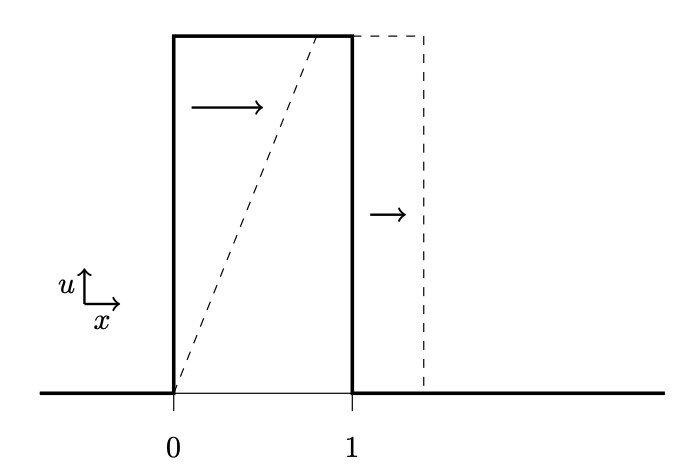
\includegraphics[width=\textwidth]{Figs/ex_set_2_3} TODO: Find the graphics for this or reproduce it (Octave or Matlab, ...)
            \caption{Initial data $u_0$, given by \eqref{eq:initial_condition}.
            The rarefaction wave and the shock both move in the positive direction.}
            \label{fig:u_0}
        \end{subfigure}
        ~
        \begin{subfigure}[b]{0.5\textwidth}
            % 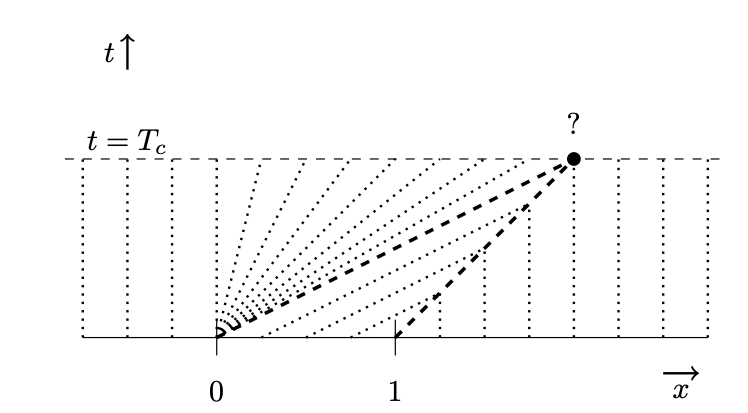
\includegraphics[width=\textwidth]{Figs/ex_set_2_2} TODO: Find the graphics for this or reproduce it (Octave or Matlab, ...)
            \caption{Characteristics of the solution of the Burger's equation
            up until time $T_c$. The rarefaction wave moves faster than
            the shock and at some point in time $t = T_c > 0$ they meet,
            and the characteristics cross each other.}
            \label{fig:characteritics}
        \end{subfigure}
        \caption{Initial condition $u_0$ and characteristics up until $T_c$.}
        \label{problem3_part1}
    \end{figure}
    
    \begin{itemize}
    \item[(a)]
    Figure \ref{problem3_part1} contains a sketch of the initial data profile
    $u_0$ with characteristics evolving. To determine
    the speed of the shock originating at $x = 1$, we use the Rankine-Hugoniot jump condition
    \begin{gather}
    	s_{shock}=\frac{f\left(u_{l}\right)-f\left(u_{r}\right)}{u_{l}-u_{r}}=\frac{\frac{1}{2} 2^{2}-\frac{1}{2}(0)^{2}}{2-(0)}=1.
    \end{gather}
    At the discontinuity at $x = 0$ we expect a rarefaction wave to arise. 
    From the general solution to the rarefaction wave, we have that the
    right front of this wave moves with a speed of $s_{rf} = f'(u_r) = 2$.
    The rarefaction wave thus moves to the right twice as fast as the
    shock wave and at some point in time the waves must meet.
    \item[(b)]
    First we seek to determine the exact solution for $0<t<T_{c}$, where $T_{c}$ is the time when the rarefaction wave catches up with the shock. The time $T_{c}$ is trivial to find: Since the position of the rarefaction front is $x_{r f}=2 t$ and the position of the shock is $x_{\text {shock }}=t+1$, we have $T_{c}+1=2 T_{c}$, namely $T_{c}=1 .$ Thus,
    $$
    u(x, t)=\left\{\begin{array}{ll}
    0 & x<0 \\
    \frac{x}{t} & 0<x<2 t \\
    2 & 2 t<x<t+1 \\
    0 & t+1<x
    \end{array}\right.
    $$
    $$
    s_{s h o c k}=\frac{f\left(u_{l}\right)-f\left(u_{r}\right)}{u_{l}-u_{r}}=\frac{\frac{1}{2} 2^{2}-\frac{1}{2}(0)^{2}}{2-(0)}=1
    $$
    \item[(c)]
    What happens at $t>T_{c} ?$ We again use the Rankine-Hugoniot jump condition, now to construct an $\mathrm{ODE}$ for the position of the shock $x_{s}$ after the rarefaction and shock wave have merged:
    $$
    \frac{d x_{s}(t)}{d t}=\frac{f\left(u_{l}\right)-f\left(u_{r}\right)}{u_{l}-u_{r}}=\frac{\frac{1}{2}\left(\frac{x_{s}(t)}{t}\right)^{2}-\frac{1}{2}(0)^{2}}{\frac{x_{s}(t)}{t}-(0)}=\frac{1}{2} \frac{x_{s}(t)}{t}
    $$
    This ODE has the general solution $x_{s}(t)=C \sqrt{t}$. At $t=1$ we know that $x_{s}=2$ so $C=2$. But what about the profile of $u(x, t) ?$ For times $t>T_{c}$, we expect the solution to the left of the shock-curve to be obtained from the rarefaction solution, i.e., $u=x / t$, while the solution on the right to be $u=0$. Note that this is compatible with the entropy condition for a shock. Thus, the solution can be expressed as
    $$
    u(x, t)=\left\{\begin{array}{ll}
    0 & x<0 \\
    \frac{x}{t} & 0<x<2 \sqrt{t} \\
    0 & x>2 \sqrt{t}
    \end{array}\right.
    $$
    Figure \ref{problem3_part2} shows the characteristic curves in the $x-t$ plane up to $t=T_{c}$ and beyond. One can see that the information originating from $(x, t)=(0,0)$ reaches up to the shock, even after the rarefaction front have caught up with it. This means that for $t>T_{c}$, in $0<x<x_{s}$, the solution is determined exclusively by the rarefaction wave, and is not affected by the location, or the existence of the shock.
    
    \begin{figure}
        \centering
        \begin{subfigure}[b]{0.5\textwidth}
            % 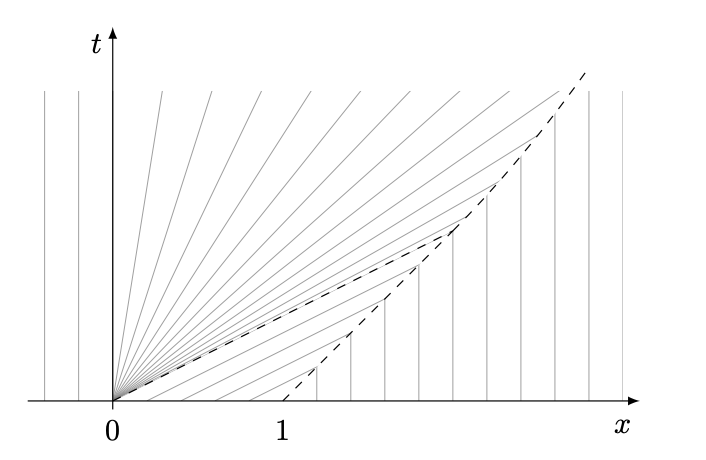
\includegraphics[width=\textwidth]{Figs/ex_set_2_4} TODO: Find the graphics for this or reproduce it (Octave or Matlab, ...)
    %        \caption{Initial data $u_0$, given by \eqref{eq:initial_condition}.
    %        The rarefaction wave and the shock both move in the positive direction.}
    %        \label{fig:u_0}
        \end{subfigure}
        \caption{The characteristic curves (gray lines) of u in the $x-t$ plane.}
        \label{problem3_part2}
    \end{figure}
    \end{itemize}
    %\begin{figure}[t!]
    %    \centering
    %    \begin{subfigure}[t]{0.5\textwidth}
    %        \centering
    %        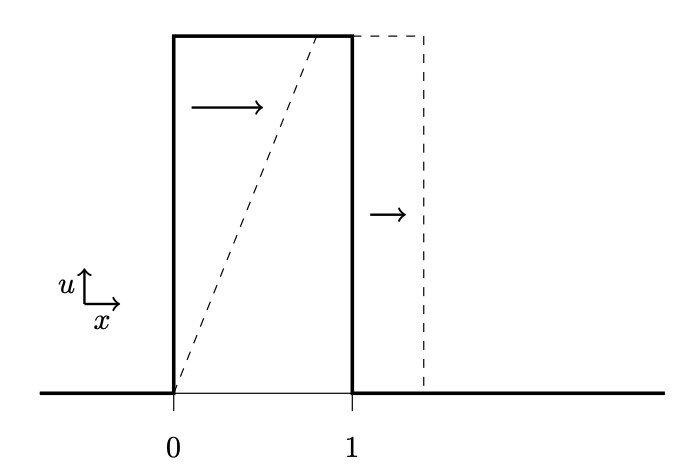
\includegraphics[height=2.5in]{Figs/ex_set_2_3}
    %        \caption{a}
    %        \label{subfig:loss_alg_2}
    %    \end{subfigure}%
    %    \\
    %    \begin{subfigure}[t]{0.5\textwidth}
    %        \centering
    %        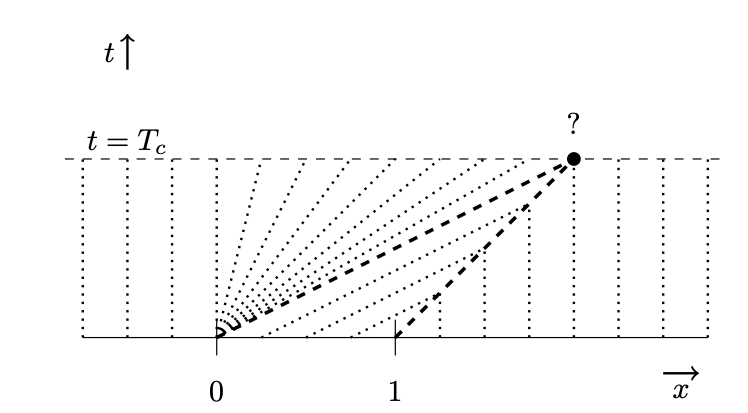
\includegraphics[height=2.5in]{Figs/ex_set_2_2}
    %        \caption{a}
    %        \label{subfig:error_alg_2}
    %    \end{subfigure}
    %    \caption{a}
    %}
    %\label{fig:alg_2}
    %\end{figure}
    
    %\begin{figure}[h!]
    %\centering
    %\begin{tikzpicture}[scale=1]
    %\draw (0,0) -- (2, 2);
    %\end{tikzpicture}
    
    %\caption{Characte}
    %\label{fig:L_domain}
    %\end{figure}
\end{solution}





\end{document}
